\chapter{جزئیات فنی پروژه}


\section{مقدمه}
در این پروژه از جهت آنکه نسخه قبلی و پیشینی برای  آن نبوده است، به ناچار می‌بایست که کد آن از صفر تا صد آن به صورت دستی نوشته شود. از این‌رو، پیچیدگی های بسیار فراوان را به طور خاص در پی داشت. ابزار های زیادی نیز بنابه شرایط در آن استفاده شد که ارتباط بین آن ابزار ها و اجزا، بر این پیچیدگی پیاده سازی طرح افزوده بود.

ابزار های اصلی و کلی که در این پروژه استفاده شده بود، عبارتند از:

\begin{itemize}
	\item 
	\textbf{نرم افزار پری اسکن}
	\LTRfootnote{PreScan}
	، نسخه \lr{$8.5.0$}
	
	\item 
	\textbf{نرم افزار قدرتمند متلب}
	\LTRfootnote{Matlab}
	، نسخه \lr{R2017b}
	\item 
	\textbf{زبان برنامه نویسی پایتون}
	، نسخه \lr{$3.6.9$}
\end{itemize}

بنابراین برای راه اندازی مجدد کد این پروژه لازم است که موارد بالا روی کامپیوتر شخص به صورت کامل نصب باشد.

همچنین لازم به ذکر است که برخی ابزارات دیگر نیز در این پروژه استفاده شده است که احتمالا با نصب موارد بالا دیگر نیازی به نصب آن ها به صورت جداگانه نیست. هدف این ابزار ها ایجاد اتصال بین اجزای اصلی گفته شده است. این گروه شامل موارد زیر هستند:

\begin{itemize}
	\item 
	\textbf{سیمولینک}
	\LTRfootnote{Simulink}
	، جهت اتصال بین متلب و پری اسکن
	
	\item 
	\textbf{شبکه \lr{UDP}}
	\RTLfootnote{برای این منظور از ماژول \lr{socket} در پایتون استفاده شده است. }
	، جهت اتصال داده های پویا 
	\LTRfootnote{Dynamic Data}
	بین پایتون و سیمولینک
	
	\item 
	\textbf{موتور متلب}
	\LTRfootnote{\matlabengine}
	، جهت اتصال داده های ساکن
	\LTRfootnote{Static Data}
	بین پایتون و سیمولینک
\end{itemize}

در این فصل جزئیات بیشتری در مورد لزوم و دلیل استفاده از این ابزار ها بررسی می‌شود.


\section{دورنمای کلی طرح}
همان‌طور که گفته شد، در این پروژه از ابزار های مختلفی استفاده شده است. برخی ابزارات دیگر نیز جهت ایجاد اتصال بین آن ابزار ها استفاده شده اند. در این بخش می‌خواهیم معرفی کنیم که 
 شکل 
\ref{fig:block-diagram}

\begin{figure}[h!]
	\centering
	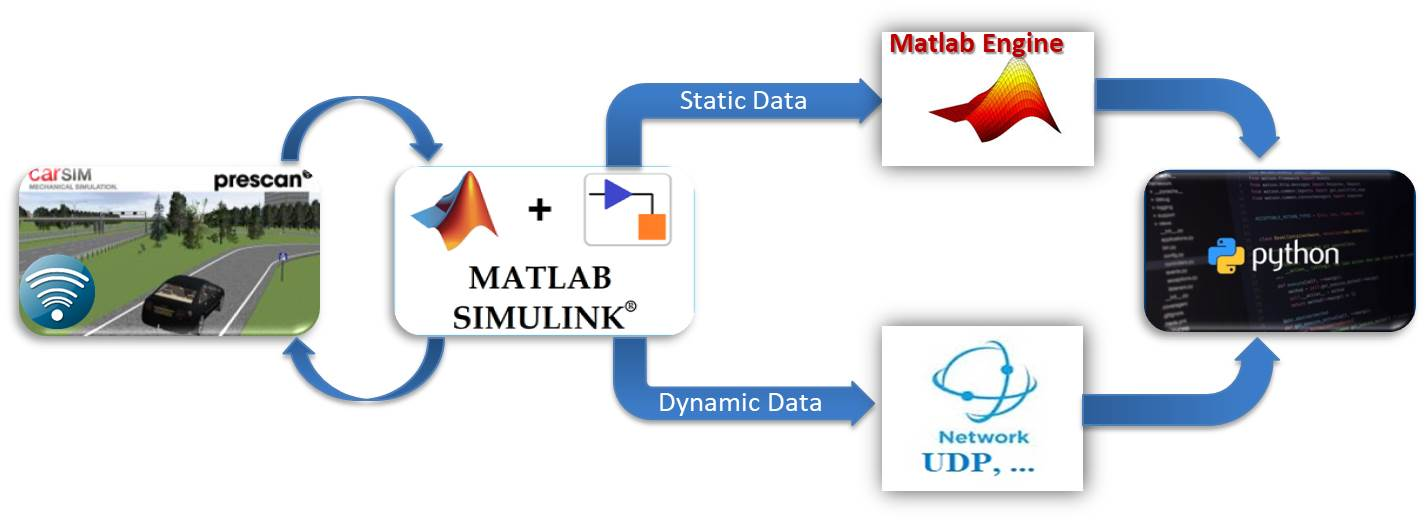
\includegraphics[width=1\linewidth]{Figures/block-diagram-white}
	\caption{بلوک دیالگرام لایه های کلی}
	\label{fig:block-diagram}
\end{figure}

\begin{figure}[h!]
	\centering
	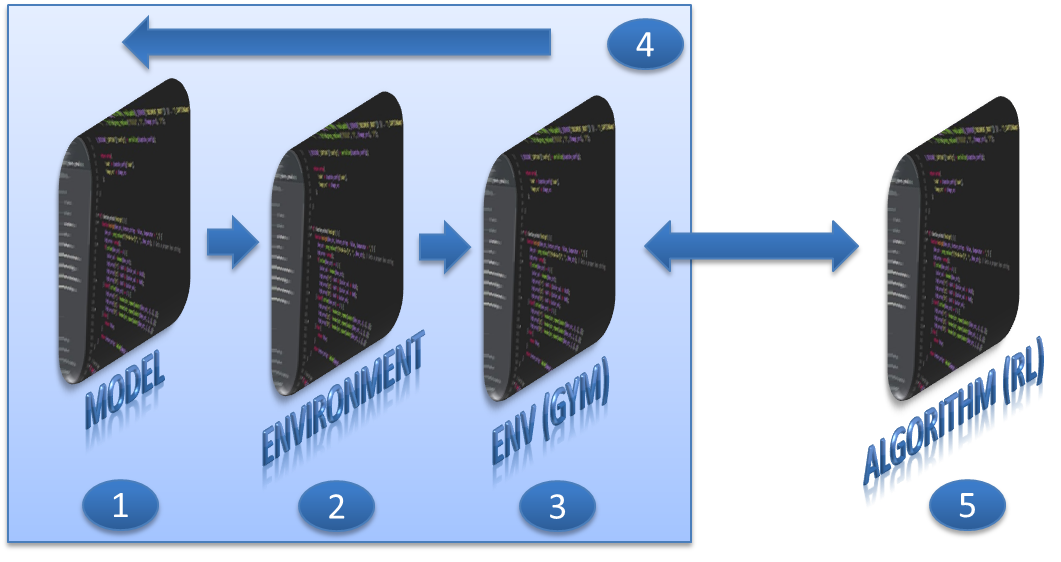
\includegraphics[width=0.7\linewidth]{Figures/python-layers-white}
	\caption{بلوک دیالگرام لایه های پایتون}
	\label{fig:python-layers}
\end{figure}






%\thispagestyle{empty}
%
%\section{مقدمه}
%
%فصل مقدمه یک پایان نامه، با بیان نیاز موضوع، تعريف مسئله و اهمیت آن در یک یا چند بند (پاراگراف) آغاز مي‌شود\footnote{شروع مقدمه نبايد چنان طولاني باشد كه هدف اصلي را تحت‌ تاثير قرار دهد.}  و با مرور پيشينه موضوع (سابقه کارهای انجام‌شده پیشین که ارتباط مستقیمی با مسئله مورد بررسی دارند) ادامه مي‌يابد. سپس در یک یا دو بند توضیح داده مي‌شود كه در این پایان نامه، چه ديدگاه يا راهكار جدیدي نسبت به مسئله (موضوع) مورد بررسي وجود دارد. به‌عبارت دیگر نوآوری‌ها به‌صورت کاملاً شفاف و صریح بیان می‌شود. در ادامه ممکن است به نتايج بدست‌آمده نیز به‌طور مختصر و کلی اشاره ‌شود. در آخرین بند از مقدمه به محتواي فصل‌هاي بعدي پایان نامه به‌اختصار اشاره مي‌شود.\\
%برای مشاهده دستورالعمل کامل دانشگاه صنعتی امیرکبیر(پلی تکنیک تهران) به \cite{zakeri} یا به سایت
%%
%\href{http://library.aut.ac.ir/Thesis%20Guide}{کتابخانه دانشگاه صنعتی امیرکبیر(پلی تکنیک تهران)}%
%مراجعه نمایید.
%
%نگارش صحيح يک پایان نامه در فهم آسان آن بسيار موثر است. در اين فصل مهمترین قواعد نگارشی که باید مورد توجه جدی نگارنده قرار گیرد، به اختصار بیان می‌شود. اين قواعد را مي‌توان در محورهای اصلی زير دسته‌بندی کرد:
%\begin{itemize}
%\item
%فارسی نویسی
%\item
%رعایت املای صحيح 
%\item
%رعایت قواعد نشانه‌گذاری
%\end{itemize}
%\section{فارسی نویسی}
%در حد امکان سعی کنيد به جاي کلمات غير‌فارسی از معادل فارسی آنها استفاده کنيد، به‌ويژه در مواردی که معادل فارسی مصطلح و رايج است‌.‌ به‌طور مثال استفاده از کلمه «لذا» به‌جای «برای همين» يا «به‌همين دليل» توجيهی ندارد‌. همچنين کلمه «پردازش» زيباتر از «پروسس» و معادل فارسی «ريز‌پردازنده» مناسب‌تر از «ميکروپروسسور» است‌.‌ در اين‌گونه موارد چنانچه احتمال عدم آشنايی خواننده با معادل فارسی وجود دارد، يا اصطلاح غير‌فارسی معمول‌تر است، در اولين ظهور کلمه فارسی، اصل غير‌فارسی آن به‌صورت پاورقي آورده شود‌.‌ اگر به‌ناچار بايد کلمات انگليسی در لابه‌لای جملات گنجانده شوند، از هر طرف يک فاصله بين آنها و کلمات فارسی پیش و پس از آنها در‌نظر گرفته شود‌.‌ چنانچه در پایان نامه از مختصر‌نويسی استفاده شود، لازم است در اولين استفاده، تفصيل آن در پاورقي آورده شود‌.‌ 
%
%\section{رعایت املای صحيح }
%رعايت املاي صحيح فارسي به مطالعه و درک راحت‌تر کمک مي‌کند. همچنين در نوشته‌هاي فارسي بايد در حد امکان از همزه « ء، أ، ؤ، ة، إ، ئ» استفاده نشود‌.‌ به‌عنوان مثال «اجزاء هواپیما» و «آئين نگارش» ناصحیح، اما «اجزاي هواپیما» و «آيين نگارش» صحيح هستند.‌
%\section{رعایت قواعد نشانه‌گذاری}
%منظور از نشانه‌گذاري به‌کار‌بردن علامت‌ها و نشانه‌هايي است که خواندن و فهم درست یک جمله را ممکن و آسان مي‌کند. در ادامه نشانه‌هاي معمول و متداول در زبان فارسي و موارد کاربرد آنها به اختصار معرفی می‌شوند.
%
%\subsection{ويرگول}
%ويرگول نشانه ضرورت یک مکث کوتاه است و در موارد زير به‌کار مي‌رود:
%\begin{itemize}
%\item
%در ميان دو کلمه که احتمال داده شود خواننده آنها را با کسره اضافه بخواند، يا نبودن ويرگول موجب بروز اشتباه در خواندن جمله شود.
%\item
%در موردي که کلمه يا عبارتي به‌‌‌‌عنوان توضيح، در ضمن یک جمله آورده شود. مثلاً برای کنترل وضعیت فضاپیماها، به‌دلیل آن‌که در خارج از جو هستند، نمی‌توان از بالک‌های آیرودینامیکی استفاده کرد.
%\item
%جدا‌کردن بخش‌هاي مختلف يک نشاني يا یک مرجع
%\item
%موارد دیگر از این قبیل
%\end{itemize}
%پیش از ويرگول نبايد فاصله گذاشته شود و پس از آن يک فاصله لازم است و بيشتر از آن صحیح نیست.
%\subsection{نقطه}
%نقطه نشانه پایان یک جمله است. پیش از نقطه نبايد فاصله گذاشته شود و پس از آن يک فاصله لازم است و بيشتر از آن صحیح نیست.
%\subsection{دونقطه}
%موارد کاربرد دونقطه عبارتند از:
%\begin{itemize}
%\item
%پيش از نقل قول مستقيم
%\item
%پيش از بيان تفصيل مطلبي که به اجمال به آن اشاره شده‌است.
%\item
%پس از واژه‌اي که معني آن در برابرش آورده و نوشته مي‌شود.
%\item
%پس از کلمات تفسير‌کننده از قبيل «يعني» و ...
%\end{itemize}
%پیش از دونقطه نبايد فاصله گذاشته شود و پس از آن يک فاصله لازم است و بيشتر از آن صحیح نیست.
%\subsection{گیومه}
%موارد کاربرد گیومه عبارتند از:
%\begin{itemize}
%\item
%وقتي که عين گفته يا نوشته کسي را در ضمن نوشته و مطلب خود مي‌آوريم. 
%\item
%در آغاز و پايان کلمات و اصطلاحات علمي و يا هر کلمه و عبارتي که بايد به‌صورت ممتاز از قسمت‌هاي ديگر نشان داده شود.
%\item
%در ذکر عنوان مقاله‌ها، رساله‌ها، اشعار، روزنامه‌ها و ...
%\end{itemize}
%\subsection{نشانه پرسشی}
%پیش از «؟» نبايد فاصله گذاشته شود و پس از آن يک فاصله لازم است و بيشتر از آن صحیح نیست.
%\subsection{خط تیره}
%موارد کاربرد خط تیره عبارتند از:
%\begin{itemize}
%\item
%جدا‌کردن عبارت‌هاي توضيحي، بدل، عطف بيان و ...
%\item
%به‌جاي حرف اضافه «تا» و «به» بين تاريخ‌ها، اعداد و کلمات
%\end{itemize}
%\subsection{پرانتز}
%موارد کاربرد پرانتز عبارتند از:
%\begin{itemize}
%\item
%به‌معني «يا» و «يعني» و وقتي که یک کلمه يا عبارت را براي توضيح بيشتر کلام بياورند.
%\item
%وقتي که نويسنده بخواهد آگاهي‌هاي بيشتر (اطلاعات تکميلي) به خواننده عرضه کند.
%\item
%براي ذکر مرجع در پايان مثال‌ها و شواهد.
%\end{itemize}
%نکته: بین کلمه یا عبارت داخل پرانتز و پرانتز باز و بسته نباید فاصله وجود داشته باشد.
%\section{جدا یا سرهم نوشتن برخی کلمات}
%تقريباً تمامي کلمات مرکب در زبان فارسي بايد از هم جدا نوشته شوند؛ به استثناي صفات فاعلي مانند «عملگر»، «باغبان» و يا «دانشمند» و کلماتي نظير «اينکه»، «آنها». در ادامه به نمونه‌هايي از مواردي که بايد اجزاي يک کلمه جدا، اما بدون فاصله نوشته شوند، اشاره مي‌شود‌:
%\begin{enumerate}
%\item
%در افعال مضارع و ماضی استمراری که با «می» شروع می‌شوند، لازم است که در عين جدا نوشتن، «می» از بخش بعدي فعل جدا نيافتد‌.‌ برای اين منظور بايد از «فاصله متصل» استفاده و «می» در اول فعل با \lr{SS}\LTRfootnote{Shift+Ctrl+@} از آن جدا شود.‌ به‌طور مثال «می‌شود» به‌جاي «می شود». 
%\item
%	«ها»ی جمع بايد از کلمه جمع بسته‌شده جدا نوشته شود؛ مگر در برخی کلمات مانند «آنها». اين امر در مورد کلمات غير‌فارسي که وارد زبان فارسي شده‌اند و با حرف «ها» جمع بسته می‌شوند، مانند «کانال‌ها» يا «فرمول‌ها» مورد تاکيد است.
%\item
%	حروف اضافه مانند «به» وقتي به‌صورت ترکيب ثابت همراه کلمه پس از خود آورده می‌شوند، بهتر است با \lr{SS} از آن جدا شوند‌.‌ مانند «به‌صورت»، «به‌عنوان» و «به‌‌‌لحاظ»‌.‌ لازم به ذکر است هنگامی که حرف اضافه «به» با کلمه پس از خود معناي قيدي داشته باشد، مثل «بشدت» يا «بسادگي»، بهتر است که به‌صورت چسبيده نوشته شود‌.
%\item
%	کلمات فارسی نبايد با قواعد عربی جمع بسته شوند؛ پس «پيشنهادها» صحيح و «پيشنهادات» اشتباه است‌.‌
%\item
%	اسم‌ها و صفت‌هاي دو‌قسمتي مثل «خط‌چين» و «نوشته‌شده» با \lr{SS} از هم جدا می‌شود‌.‌
%\item
%	شناسه‌ها با \lr{SS} از کلمه اصلي جدا می‌شود‌.‌ مثل «شده‌اند»‌ و «شده‌است». 
%\item
%	‌ «است» هنگامی که نقش شناسه را داشته باشد توسط \lr{SS} از قسمت اصلي جدا می‌شود‌.‌ مانند «گفته‌است»‌.
%\item
%	بند پیشین نبايد باعث افراط در استفاده از فاصله متصل شود. مثلاً عبارت «نوشته می‌شود‌« صحيح و عبارت «نوشته‌می‌شود» ناصحیح است. 
%\item
%	فعل‌هاي دو‌کلمه‌اي که معناي اجزاي آنها کاملاً با معناي کل متفاوت است، بهتر است که با \lr{SS} از هم جدا ‌شوند‌.‌
%\item
%	کلمات مرکب مثل کلمه «دوکلمه‌اي» در عبارت «فعل‌هاي دوکلمه‌اي» و «يادداشت‌برداري».
%\item
%	مصدرهاي دو قسمتي با \lr{SS} از هم جدا می‌شوند‌.‌ مثل «ذوب‌کردن» و «واردکردن»‌.
%\item
%	 صفات تفضيلي مثل « آسان‌تر».
%\end{enumerate}
%
